\chapter{Polímeros: síntese, estrutura e propriedades}\label{ch:b2:polymer-synthesis}

As meias de náilon foram postas à venda em 1939. Elas saíram de um laboratório que se propusera, alguns
anos antes, a compreender como pequenas moléculas se unem em moléculas longas, e que aprendera no
caminho uma lição que surpreende todo químico na primeira vez: para um \omterm{def:b2:polymer-synthesis:polymer}{polímero} feito unindo moléculas
ponta a ponta, um rendimento de 99~\% não basta. Este capítulo explica por quê, descreve as duas
maneiras pelas quais as cadeias crescem e liga a estrutura das cadeias às propriedades dos materiais.
% ledger: hist:nylon-production-1939

\begin{recall}
O volume escolar: \omterm{def:b2:polymer-synthesis:polymer}{polímeros}, \omterm{def:b2:polymer-synthesis:polymer}{monômeros} e \omterm{def:b2:polymer-synthesis:polymer}{unidades de repetição}, \omterm{def:b2:polymer-synthesis:polymer}{polímeros} de adição e de condensação,
termoplásticos e termorrígidos. O volume do 1.º ano: radicais e homólise, carbocátions e carbânions, a
aproximação do estado estacionário. \Cref{ch:b2:acyl-substitution}: ésteres e amidas.
\Cref{ch:b2:catalytic-cycles}: a inserção em uma ligação metal--carbono.
\end{recall}

\section{As cadeias e suas massas molares}

\begin{definition}[Polímero]\label{def:b2:polymer-synthesis:polymer}
Um \emph{polímero}\index{polimero@polímero} é uma substância formada por macromoléculas, cada uma construída pela
ligação repetida de pequenas moléculas, os \emph{monômeros}\index{monomero@monômero}. A \emph{unidade de repetição}\index{unidade de repeticao@unidade de repetição}
é o menor grupo de átomos cuja repetição compõe a cadeia; o \emph{grau de
polimerização}\index{grau de polimerizacao@grau de polimerização} $X$ de uma cadeia é o número de unidades provenientes de monômeros
que ela contém.
\end{definition}

Uma amostra de um \omterm{def:b2:polymer-synthesis:polymer}{polímero} sintético nunca é feita de cadeias idênticas: é uma mistura de cadeias de
comprimentos diferentes, e sua massa molar é uma média, que depende da maneira de contar as cadeias.

\begin{definition}[Massas molares médias]\label{def:b2:polymer-synthesis:averages}
Para uma amostra que contém $N_i$ cadeias de massa molar $M_i$, a \emph{massa molar média em
número}\index{massa molar media em numero@massa molar média em número} e a \emph{massa molar média em massa}\index{massa molar media em massa@massa molar média em massa}
são
\begin{equation*}
\bar M_n = \frac{\sum_i N_i M_i}{\sum_i N_i}, \qquad
\bar M_w = \frac{\sum_i N_i M_i^2}{\sum_i N_i M_i} = \sum_i w_i M_i,
\end{equation*}
onde $w_i$ é a fração mássica das cadeias de massa $M_i$. A \emph{dispersidade}\index{dispersidade}
$\text{\DH} = \bar M_w/\bar M_n$ é no mínimo 1, e igual a 1 somente se todas as cadeias têm a mesma
massa. As médias $\bar X_n$ e $\bar X_w$ do \omterm{def:b2:polymer-synthesis:polymer}{grau de polimerização} são definidas da mesma
maneira.
\end{definition}

A média em número pesa cada cadeia uma vez; a média em massa pesa cada cadeia por sua massa, de modo que
as cadeias longas contam mais. Que $\text{\DH} \ge 1$ é a desigualdade $\left(\sum N_i M_i\right)^2 \le
\sum N_i \sum N_i M_i^2$ (Cauchy--Schwarz), com igualdade só para $M_i$ iguais.

\begin{method}[Calcular as médias]\label{met:b2:polymer-synthesis:averages}
\begin{enumerate}
  \item Converta os dados em quantidades $N_i$ (ou números de cadeias) e massas $M_i$; a partir das
        frações mássicas, $N_i \propto w_i/M_i$.
  \item $\bar M_n = \sum N_i M_i / \sum N_i$; de modo equivalente, $1/\bar M_n = \sum w_i/M_i$.
  \item $\bar M_w = \sum w_i M_i$.
  \item $\text{\DH} = \bar M_w/\bar M_n$; verifique que $\bar M_w \ge \bar M_n$.
\end{enumerate}
\end{method}

\section{Crescimento em etapas e crescimento em cadeia}

\begin{definition}[Crescimento em etapas e em cadeia]\label{def:b2:polymer-synthesis:step-chain}
Em uma \emph{polimerização em etapas}\index{polimerizacao em etapas@polimerização em etapas}, duas moléculas quaisquer que levam
grupos funcionais complementares (\omterm{def:b2:polymer-synthesis:polymer}{monômeros}, oligômeros ou cadeias longas) podem reagir, e as cadeias
se alongam unindo-se umas às outras: poliésteres, poliamidas. Em uma \emph{polimerização em
cadeia}\index{polimerizacao em cadeia@polimerização em cadeia}, um centro reativo (radical, íon ou ligação metal--carbono)
acrescenta moléculas de \omterm{def:b2:polymer-synthesis:polymer}{monômero} uma de cada vez à extremidade de uma cadeia em crescimento: os
\omterm{def:b2:polymer-synthesis:polymer}{polímeros} dos alcenos.
\end{definition}

\begin{method}[Em etapas ou em cadeia?]\label{met:b2:polymer-synthesis:classify}
\begin{enumerate}
  \item Um \omterm{def:b2:polymer-synthesis:polymer}{monômero} com dois grupos funcionais que reagem com o parceiro um do outro (ácido e álcool,
        ácido e amina), muitas vezes liberando uma pequena molécula: crescimento em etapas.
  \item Um \omterm{def:b2:polymer-synthesis:polymer}{monômero} com uma ligação dupla \ce{C=C} (ou um anel tensionado) e um iniciador: crescimento
        em cadeia.
  \item Confira com o curso da reação: no crescimento em etapas, o \omterm{def:b2:polymer-synthesis:polymer}{monômero} desaparece cedo e as
        cadeias longas só aparecem no final; no crescimento em cadeia, cadeias longas aparecem desde o
        início enquanto o \omterm{def:b2:polymer-synthesis:polymer}{monômero} é consumido aos poucos.
\end{enumerate}
\end{method}

\subsection*{Crescimento em etapas}

Tome uma mistura equilibrada de \omterm{def:b2:polymer-synthesis:polymer}{monômeros} \ce{A-A} e \ce{B-B} (uma diamina e um diácido), ou um único
\omterm{def:b2:polymer-synthesis:polymer}{monômero} \ce{A-B}. Chame de $p$ o \emph{grau de avanço}: a fração dos grupos funcionais de um mesmo
tipo que reagiram.

\begin{theorem}[Equação de Carothers]\label{thm:b2:polymer-synthesis:carothers}
Em uma \omterm{def:b2:polymer-synthesis:step-chain}{polimerização em etapas} de \omterm{def:b2:polymer-synthesis:polymer}{monômeros} bifuncionais exatamente equilibrados, o \omterm{def:b2:polymer-synthesis:polymer}{grau de
polimerização} médio em número, contado em unidades de \omterm{def:b2:polymer-synthesis:polymer}{monômero}, é
\begin{equation*}
\bar X_n = \frac{1}{1 - p}.
\end{equation*}
\end{theorem}

\begin{proof}
Partimos de $N_0$ moléculas de \omterm{def:b2:polymer-synthesis:polymer}{monômero}, que levam $N_0$ grupos \ce{A} e $N_0$ grupos \ce{B}. Cada
reação entre um \ce{A} e um \ce{B} une duas moléculas em uma, portanto diminui o número de moléculas
de uma unidade. Após $pN_0$ reações restam $N = N_0 - pN_0 = N_0(1-p)$ moléculas que compartilham as $N_0$
unidades de \omterm{def:b2:polymer-synthesis:polymer}{monômero}: $\bar X_n = N_0/N = 1/(1-p)$.
\end{proof}

\begin{corollary}[Desequilíbrio]\label{cor:b2:polymer-synthesis:imbalance}
Se os grupos não estão equilibrados, com $r = N_{\ce{A}}/N_{\ce{B}} \le 1$ e $p$ o grau de avanço dos
grupos minoritários \ce{A},
\begin{equation*}
\bar X_n = \frac{1 + r}{1 + r - 2rp}, \qquad \text{no máximo } \frac{1+r}{1-r} \text{ quando } p = 1.
\end{equation*}
\end{corollary}

\begin{proof}
Há no início $(N_{\ce{A}} + N_{\ce{B}})/2$ moléculas de \omterm{def:b2:polymer-synthesis:polymer}{monômero} bifuncionais. Cada molécula
linear tem duas extremidades de cadeia, cada uma um grupo que não reagiu; após a reação restam $N_{\ce{A}}(1-p)$
grupos \ce{A} e $N_{\ce{B}} - pN_{\ce{A}}$ grupos \ce{B}, logo $N = [N_{\ce{A}}(1-p) + N_{\ce{B}} -
pN_{\ce{A}}]/2$ moléculas. Dividindo, com $N_{\ce{B}} = N_{\ce{A}}/r$:
$\bar X_n = (1 + 1/r)/(1 - 2p + 1/r) = (1+r)/(1 + r - 2rp)$. Com $r = 1$, esta é a equação de Carothers.
\end{proof}

A equação explica a frase de abertura. Com $p = 0.99$, um ``rendimento de 99~\%'' da reação de ligação, $\bar X_n =
100$; uma fibra útil precisa de cerca disso ou mais, de modo que a ligação deve ir além de 99~\%, com
\omterm{def:b2:polymer-synthesis:polymer}{monômeros} puros em quantidades exatamente iguais e a pequena molécula liberada (água, metanol) removida
para continuar deslocando o equilíbrio. Um excesso de 1~\% de um \omterm{def:b2:polymer-synthesis:polymer}{monômero} limita $\bar X_n$ a 201 mesmo
com \omterm{def:b2:continuous-reactors:conversion}{conversão} completa.

\begin{theorem}[Distribuição de Flory]\label{thm:b2:polymer-synthesis:flory}
Em uma \omterm{def:b2:polymer-synthesis:step-chain}{polimerização em etapas} com grau de avanço $p$, se todo grupo tem a mesma reatividade qualquer que
seja o comprimento de sua cadeia, a fração em número e a fração mássica das cadeias de $x$ unidades são
\begin{equation*}
n_x = (1-p)\,p^{\,x-1}, \qquad w_x = x(1-p)^2 p^{\,x-1},
\end{equation*}
e $\bar X_n = 1/(1-p)$, $\bar X_w = (1+p)/(1-p)$, de modo que $\text{\DH} = 1 + p$, perto de 2 com
\omterm{def:b2:continuous-reactors:conversion}{conversão} elevada.
\end{theorem}

\begin{proof}
Siga uma cadeia a partir de uma extremidade (um \omterm{def:b2:polymer-synthesis:polymer}{monômero} \ce{A-B}, para simplificar). Cada ligação ao
longo dela é formada com probabilidade $p$, de modo independente. A cadeia tem exatamente $x$ unidades
se as $x-1$ primeiras ligações estão formadas e a seguinte não: probabilidade $p^{\,x-1}(1-p)$, que é $n_x$. Com $\sum_{x\ge1} p^{\,x-1} =
1/(1-p)$ e suas derivadas $\sum x p^{\,x-1} = 1/(1-p)^2$ e $\sum x^2 p^{\,x-1} = (1+p)/(1-p)^3$:
$\sum n_x = 1$, $\bar X_n = \sum x n_x = 1/(1-p)$, $w_x = x n_x/\bar X_n = x(1-p)^2p^{\,x-1}$, e
$\bar X_w = \sum x w_x = (1-p)^2(1+p)/(1-p)^3 = (1+p)/(1-p)$.
\end{proof}

\begin{omfigure}
\begin{tikzpicture}
\begin{axis}[width=0.46\linewidth, height=5cm, xmin=0, xmax=400, ymin=0,
  xlabel={grau de polimerização $x$}, ylabel={fração mássica $w_x$}, label style={font=\small},
  tick label style={font=\scriptsize}, scaled y ticks=false,
  yticklabel style={/pgf/number format/fixed, /pgf/number format/precision=3},
  legend style={font=\scriptsize, at={(0.98,0.98)}, anchor=north east}, legend cell align=left]
\addplot[omDef, thick] table[x=x, y=p95] {figdata/out/bachelor-2-polymer-distributions-a.dat};
\addplot[omThm, thick] table[x=x, y=p98] {figdata/out/bachelor-2-polymer-distributions-a.dat};
\addplot[omMeth, thick] table[x=x, y=p99] {figdata/out/bachelor-2-polymer-distributions-a.dat};
\legend{$p = 0.95$, $p = 0.98$, $p = 0.99$}
\end{axis}
\end{tikzpicture}\hfill
\begin{tikzpicture}
\begin{axis}[width=0.46\linewidth, height=5cm, xmin=0, xmax=1, ymin=0, ymax=200,
  xlabel={grau de avanço $p$}, ylabel={$\bar X_n$}, label style={font=\small},
  tick label style={font=\scriptsize}, xtick={0,0.2,0.4,0.6,0.8,1}]
\addplot[omDef, thick] table[x=p, y=Xn] {figdata/out/bachelor-2-polymer-distributions-b.dat};
\end{axis}
\end{tikzpicture}

{\small \omterm{def:b2:polymer-synthesis:step-chain}{Polimerização em etapas} (modelos). À esquerda: distribuições mássicas de Flory
(\cref{thm:b2:polymer-synthesis:flory}); o pico fica perto de $\bar X_n$ e a distribuição se alarga à
medida que ele se afasta. À direita: a equação de Carothers; $\bar X_n$ continua pequeno até que $p$
esteja muito perto de 1.}
% figdata: bachelor-2/polymer-distributions.py parts a, b
\end{omfigure}

\subsection*{Crescimento radicalar em cadeia}

\begin{definition}[Etapas de uma polimerização em cadeia]\label{def:b2:polymer-synthesis:chain-steps}
Uma polimerização radicalar em cadeia ocorre em três tipos de etapas. Na \emph{iniciação}\index{iniciacao@iniciação}, um
\emph{iniciador radicalar}\index{iniciador radicalar} (uma molécula com uma ligação fraca, como um peróxido ou um
composto azo) se cinde por aquecimento em radicais, um dos quais se adiciona a um \omterm{def:b2:polymer-synthesis:polymer}{monômero}. Na
\emph{propagação}\index{propagacao@propagação}, o radical na extremidade da cadeia adiciona uma molécula de \omterm{def:b2:polymer-synthesis:polymer}{monômero} e
continua sendo um radical. Na \emph{terminação}\index{terminacao@terminação}, dois radicais se destroem mutuamente, por
combinação (eles se ligam) ou desproporcionamento (um toma um átomo de hidrogênio do outro).
\end{definition}

\begin{omfigure}
\begin{align*}
&\text{iniciação:} && \mathrm{I{-}I} \longrightarrow 2\,\mathrm{I^{\bullet}}, \qquad
\mathrm{I^{\bullet} + CH_2{=}CHPh \longrightarrow I{-}CH_2{-}\dot{C}HPh} \\
&\text{propagação:} && {\sim}\mathrm{CH_2{-}\dot{C}HPh + CH_2{=}CHPh \longrightarrow}\;
{\sim}\mathrm{CH_2{-}CHPh{-}CH_2{-}\dot{C}HPh} \\
&\text{terminação:} && {\sim}\mathrm{CH_2{-}\dot{C}HPh + Ph\dot{C}H{-}CH_2}{\sim} \longrightarrow
{\sim}\mathrm{CH_2{-}CHPh{-}CHPh{-}CH_2}{\sim}
\end{align*}

{\small Polimerização radicalar do estireno. O iniciador \ce{I-I} (peróxido de dibenzoíla, por exemplo)
se cinde em dois radicais; cada um se adiciona à extremidade \ce{CH2} do estireno, dando o radical
benzílico, mais estável; a \omterm{def:b2:polymer-synthesis:chain-steps}{propagação} repete a adição milhares de vezes; dois radicais de cadeia se
combinam e terminam ambas as cadeias. O ponto marca o elétron desemparelhado.}
\end{omfigure}

\begin{theorem}[Velocidade da polimerização radicalar]\label{thm:b2:polymer-synthesis:radical-rate}
Com um iniciador que se decompõe com constante de velocidade $k_d$ e eficiência $f$ (a fração dos
radicais que iniciam uma cadeia), constante de \omterm{def:b2:polymer-synthesis:chain-steps}{propagação} $k_p$ e constante de \omterm{def:b2:polymer-synthesis:chain-steps}{terminação} $k_t$
(velocidade de \omterm{def:b2:polymer-synthesis:chain-steps}{terminação} $2k_t
[\mathrm{M^\bullet}]^2$), a velocidade de polimerização no estado estacionário é
\begin{equation*}
R_p = k_p [\mathrm M] \sqrt{\frac{f k_d [\mathrm I]}{k_t}}.
\end{equation*}
\end{theorem}

\begin{proof}
Seja $[\mathrm{M^\bullet}]$ a concentração total de radicais de cadeia, qualquer que seja seu
comprimento. Eles são criados à velocidade $R_i = 2fk_d[\mathrm I]$ (dois radicais por molécula de
iniciador, uma fração $f$ dos quais inicia cadeias) e destruídos à velocidade $2k_t[\mathrm{M^\bullet}]^2$;
a \omterm{def:b2:polymer-synthesis:chain-steps}{propagação} transforma um radical de cadeia em outro e não muda seu número. A aproximação do estado
estacionário aplicada a
$[\mathrm{M^\bullet}]$ dá $2fk_d[\mathrm I] = 2k_t[\mathrm{M^\bullet}]^2$, logo $[\mathrm{M^\bullet}] =
\sqrt{fk_d[\mathrm I]/k_t}$. O \omterm{def:b2:polymer-synthesis:polymer}{monômero} é consumido essencialmente pela \omterm{def:b2:polymer-synthesis:chain-steps}{propagação}, a $R_p =
k_p[\mathrm M][\mathrm{M^\bullet}]$.
\end{proof}

\begin{definition}[Comprimento de cadeia cinético]\label{def:b2:polymer-synthesis:chain-length}
O \emph{comprimento de cadeia cinético}\index{comprimento de cadeia cinetico@comprimento de cadeia cinético} $\nu$ é o número médio de moléculas de
\omterm{def:b2:polymer-synthesis:polymer}{monômero} adicionadas por radical que inicia uma cadeia: $\nu = R_p/R_i$.
\end{definition}

\begin{proposition}[Comprimento de cadeia e iniciador]\label{prop:b2:polymer-synthesis:chain-length}
No estado estacionário, $\nu = k_p[\mathrm M]/\bigl(2\sqrt{fk_dk_t[\mathrm I]}\bigr)$: mais iniciador
dá uma polimerização mais rápida mas cadeias mais curtas. Com \omterm{def:b2:polymer-synthesis:chain-steps}{terminação} por combinação, $\bar X_n = 2\nu$;
por desproporcionamento, $\bar X_n = \nu$.
\end{proposition}

\begin{proof}
$\nu = R_p/R_i = k_p[\mathrm M]\sqrt{fk_d[\mathrm I]/k_t}/(2fk_d[\mathrm I]) =
k_p[\mathrm M]/\bigl(2\sqrt{fk_dk_t[\mathrm I]}\bigr)$. Cada cadeia iniciada adiciona em média $\nu$
\omterm{def:b2:polymer-synthesis:polymer}{monômeros}; a combinação une duas dessas cadeias em uma molécula, o desproporcionamento deixa duas.
\end{proof}

\begin{definition}[Polimerização viva]\label{def:b2:polymer-synthesis:living}
Uma \emph{polimerização viva}\index{polimerizacao viva@polimerização viva} é uma \omterm{def:b2:polymer-synthesis:step-chain}{polimerização em cadeia} sem
\omterm{def:b2:polymer-synthesis:chain-steps}{terminação} nem transferência: todas as cadeias começam juntas e continuam crescendo enquanto resta
\omterm{def:b2:polymer-synthesis:polymer}{monômero}, e retomam o crescimento quando se acrescenta mais \omterm{def:b2:polymer-synthesis:polymer}{monômero}. A polimerização aniônica do
estireno iniciada pelo butil-lítio em solvente anidro e aprótico é o exemplo clássico.
\end{definition}

\begin{proposition}[Distribuições estreitas]\label{prop:b2:polymer-synthesis:living}
Em uma \omterm{def:b2:polymer-synthesis:living}{polimerização viva} na qual todas as cadeias começam ao mesmo tempo, o \omterm{def:b2:polymer-synthesis:polymer}{grau de polimerização} segue
uma distribuição de Poisson, e $\text{\DH} = 1 + \nu/(1+\nu)^2 \approx 1 + 1/\bar X_n$, onde $\nu$ é o
número médio de \omterm{def:b2:polymer-synthesis:polymer}{monômeros} adicionados por cadeia.
\end{proposition}

\admitted

A distribuição é a do número de adições, eventos aleatórios independentes a uma taxa comum, feitas por
cada cadeia durante o mesmo tempo; a \omterm{def:b2:polymer-synthesis:averages}{dispersidade} decorre da média e da variância de uma lei de Poisson,
ambas iguais a $\nu$. Uma cadeia viva de 100 unidades tem assim $\text{\DH} \approx 1.01$, contra quase 2
para a mesma média obtida por crescimento em etapas.

\begin{omfigure}
\begin{tikzpicture}
\begin{axis}[width=0.72\linewidth, height=5cm, xmin=0, xmax=150, ymin=0,
  xlabel={grau de polimerização $x$}, ylabel={fração mássica $w_x$}, label style={font=\small},
  tick label style={font=\scriptsize}, scaled y ticks=false,
  yticklabel style={/pgf/number format/fixed, /pgf/number format/precision=3},
  legend style={font=\scriptsize, at={(0.98,0.98)}, anchor=north east}, legend cell align=left]
\addplot[omThm, thick] table[x=x, y=poisson] {figdata/out/bachelor-2-polymer-distributions-c.dat};
\addplot[omDef, thick] table[x=x, y=flory] {figdata/out/bachelor-2-polymer-distributions-c.dat};
\legend{viva (Poisson), em etapas (Flory)}
\end{axis}
\end{tikzpicture}

{\small Duas amostras com o mesmo $\bar X_n = 50$ (modelos). As cadeias vivas se agrupam em torno de 50 ($\text{\DH}
\approx 1.02$); as cadeias de crescimento em etapas se espalham do \omterm{def:b2:polymer-synthesis:polymer}{monômero} até várias centenas de
unidades ($\text{\DH} \approx
1.98$).}
% figdata: bachelor-2/polymer-distributions.py part c
\end{omfigure}

\begin{definition}[Copolímero]\label{def:b2:polymer-synthesis:copolymer}
Um \emph{copolímero}\index{copolimero@copolímero} é um \omterm{def:b2:polymer-synthesis:polymer}{polímero} construído a partir de dois ou mais \omterm{def:b2:polymer-synthesis:polymer}{monômeros} diferentes.
Suas unidades podem se suceder ao acaso (copolímero estatístico), de modo alternado, em longas
sequências de cada um (copolímero em blocos, obtido por \omterm{def:b2:polymer-synthesis:living}{polimerização viva}), ou como cadeias laterais de
um enxertadas em uma cadeia principal do outro (copolímero enxertado).
\end{definition}

\section{A estrutura das cadeias}

\begin{definition}[Taticidade]\label{def:b2:polymer-synthesis:tacticity}
Em um \omterm{def:b2:polymer-synthesis:polymer}{polímero} vinílico \ce{-[CH2-CHR]_n-}, cada carbono \ce{CHR} é um estereocentro. A
\emph{taticidade}\index{taticidade} descreve suas configurações relativas ao longo da cadeia desenhada em
zigue-zague plano: em uma cadeia \emph{isotática}\index{isotatica@isotática} todos os grupos \ce{R} ficam do mesmo
lado do plano, em uma cadeia \emph{sindiotática}\index{sindiotatica@sindiotática} eles se alternam, e em uma cadeia
\emph{atática}\index{atatica@atática} eles estão dispostos ao acaso.
\end{definition}

\begin{omfigure}
\setchemfig{atom sep=1.5em}
\begin{tabular}{rl}
\small \omterm{def:b2:polymer-synthesis:tacticity}{isotática} & \chemfig{[:-30]-[:30](<[:90])-[:-30]-[:30](<[:90])-[:-30]-[:30](<[:90])-[:-30]-[:30](<[:90])-[:-30]-[:30](<[:90])-[:-30]} \\[2pt]
\small \omterm{def:b2:polymer-synthesis:tacticity}{sindiotática} & \chemfig{[:-30]-[:30](<[:90])-[:-30]-[:30](<:[:90])-[:-30]-[:30](<[:90])-[:-30]-[:30](<:[:90])-[:-30]-[:30](<[:90])-[:-30]} \\[2pt]
\small \omterm{def:b2:polymer-synthesis:tacticity}{atática} & \chemfig{[:-30]-[:30](<[:90])-[:-30]-[:30](<[:90])-[:-30]-[:30](<:[:90])-[:-30]-[:30](<[:90])-[:-30]-[:30](<:[:90])-[:-30]}
\end{tabular}
\par\vspace{6pt}

{\small O polipropeno desenhado em zigue-zague no plano da página; cada grupo metila é uma cunha
(voltada para o leitor) ou uma cunha tracejada (afastada). \omterm{def:b2:polymer-synthesis:tacticity}{Isotático}: todas as metilas de um lado;
\omterm{def:b2:polymer-synthesis:tacticity}{sindiotático}: alternadas; \omterm{def:b2:polymer-synthesis:tacticity}{atático}: irregular.}
\end{omfigure}

As cadeias regulares podem se empacotar lado a lado em regiões cristalinas; as irregulares não. O
polipropeno \omterm{def:b2:polymer-synthesis:tacticity}{isotático}, obtido com os catalisadores metálicos do volume do 3.º ano, é parcialmente
cristalino, duro e de alto ponto de fusão; o polipropeno \omterm{def:b2:polymer-synthesis:tacticity}{atático} é um material amorfo mole e pegajoso.
Um \omterm{def:b2:polymer-synthesis:polymer}{polímero} raramente é totalmente cristalino: os cristalitos estão imersos em regiões amorfas onde as
cadeias estão emaranhadas.

\begin{definition}[Transições térmicas]\label{def:b2:polymer-synthesis:transitions}
O \emph{grau de cristalinidade}\index{grau de cristalinidade} de um \omterm{def:b2:polymer-synthesis:polymer}{polímero} é a fração mássica dele que se encontra
em regiões cristalinas. A \emph{temperatura de transição vítrea}\index{temperatura de transicao vitrea@temperatura de transição vítrea}
$T_g$ é a temperatura abaixo da qual as regiões amorfas são um vidro rígido, com os segmentos de cadeia
incapazes de se mover, e acima da qual elas se tornam borrachosas; as regiões cristalinas fundem a uma
temperatura mais alta, $T_m$.
\end{definition}

O poliestireno e o poli(metacrilato de metila) são amorfos com $T_g$ acima da temperatura ambiente:
vidros rígidos e transparentes. A borracha natural tem $T_g$ bem abaixo da temperatura ambiente. O
polieteno, com $T_g$ muito abaixo da temperatura ambiente mas altamente cristalino, é tenaz e flexível:
seus cristalitos mantêm unidas as partes amorfas borrachosas.

\begin{omfigure}
\begin{tikzpicture}[x=1cm, y=1cm]
\draw[->] (0,0) -- (8.6,0) node[below left, font=\small] {temperatura};
\draw[->] (0,0) -- (0,4.6) node[above, font=\small] {$\log$ módulo};
\draw[omDef, very thick] (0.2,4) .. controls (1.8,3.95) and (2.4,3.9) .. (2.8,3.6)
  .. controls (3.3,3.0) and (3.4,1.9) .. (4.0,1.75) -- (6.0,1.6)
  .. controls (6.7,1.5) and (7.0,0.8) .. (7.8,0.35);
\draw[omThm, very thick, dashed] (4.0,1.75) -- (6.0,1.7) .. controls (6.6,1.68) and (7.2,1.65) .. (8.2,1.6);
\draw[densely dotted] (3.2,0) node[below, font=\small] {$T_g$} -- (3.2,4.2);
\node[font=\footnotesize, align=center] at (1.4,3.4) {vítreo};
\node[font=\footnotesize, align=center] at (4.0,3.3) {transição};
\node[font=\footnotesize, align=center] at (5.0,2.3) {patamar borrachoso};
\node[font=\footnotesize, align=center, omDef] at (7.6,1.15) {escoa};
\node[font=\footnotesize, align=center, omThm] at (7.7,2.0) {reticulado};
\end{tikzpicture}
\par\vspace{4pt}

{\small Módulo (rigidez) de um \omterm{def:b2:polymer-synthesis:polymer}{polímero} amorfo em função da temperatura, esquema. Abaixo de $T_g$ o
material é um vidro; ao longo da transição o módulo cai várias ordens de grandeza; no patamar
borrachoso as cadeias emaranhadas se comportam como uma borracha; a temperatura mais alta, um \omterm{def:b2:polymer-synthesis:polymer}{polímero}
linear escoa (linha cheia), enquanto um reticulado conserva seu patamar até se decompor (tracejado).}
\end{omfigure}

\section{Propriedades e usos}

\begin{definition}[Elastômero]\label{def:b2:polymer-synthesis:elastomer}
Um \emph{elastômero}\index{elastomero@elastômero} é um \omterm{def:b2:polymer-synthesis:polymer}{polímero} usado acima de sua \omterm{def:b2:polymer-synthesis:transitions}{temperatura de transição vítrea}
cujas cadeias são levemente reticuladas: ele pode ser esticado a várias vezes seu comprimento e
retoma sua forma quando liberado.
\end{definition}

As quatro grandes classes de materiais poliméricos decorrem da estrutura e das transições. Os
termoplásticos, lineares ou ramificados, vítreos ou semicristalinos à temperatura ambiente, amolecem
com o aquecimento e podem ser moldados várias vezes: polieteno, polipropeno, poliestireno, PET. Os
\omterm{def:b2:polymer-synthesis:elastomer}{elastômeros} são cadeias levemente reticuladas acima de sua $T_g$: a borracha vulcanizada, na qual
pontes de enxofre ligam as cadeias. As fibras são cadeias alinhadas por estiramento, com fortes
interações entre elas: as ligações de hidrogênio entre os grupos amida no náilon. Os termorrígidos são
redes densamente reticuladas formadas durante a moldagem: resinas epóxi e fenol--formaldeído, que não
podem ser refundidas. Só os termoplásticos são reciclados por fusão; o volume escolar deu a dimensão do
problema.

\begin{omfigure}
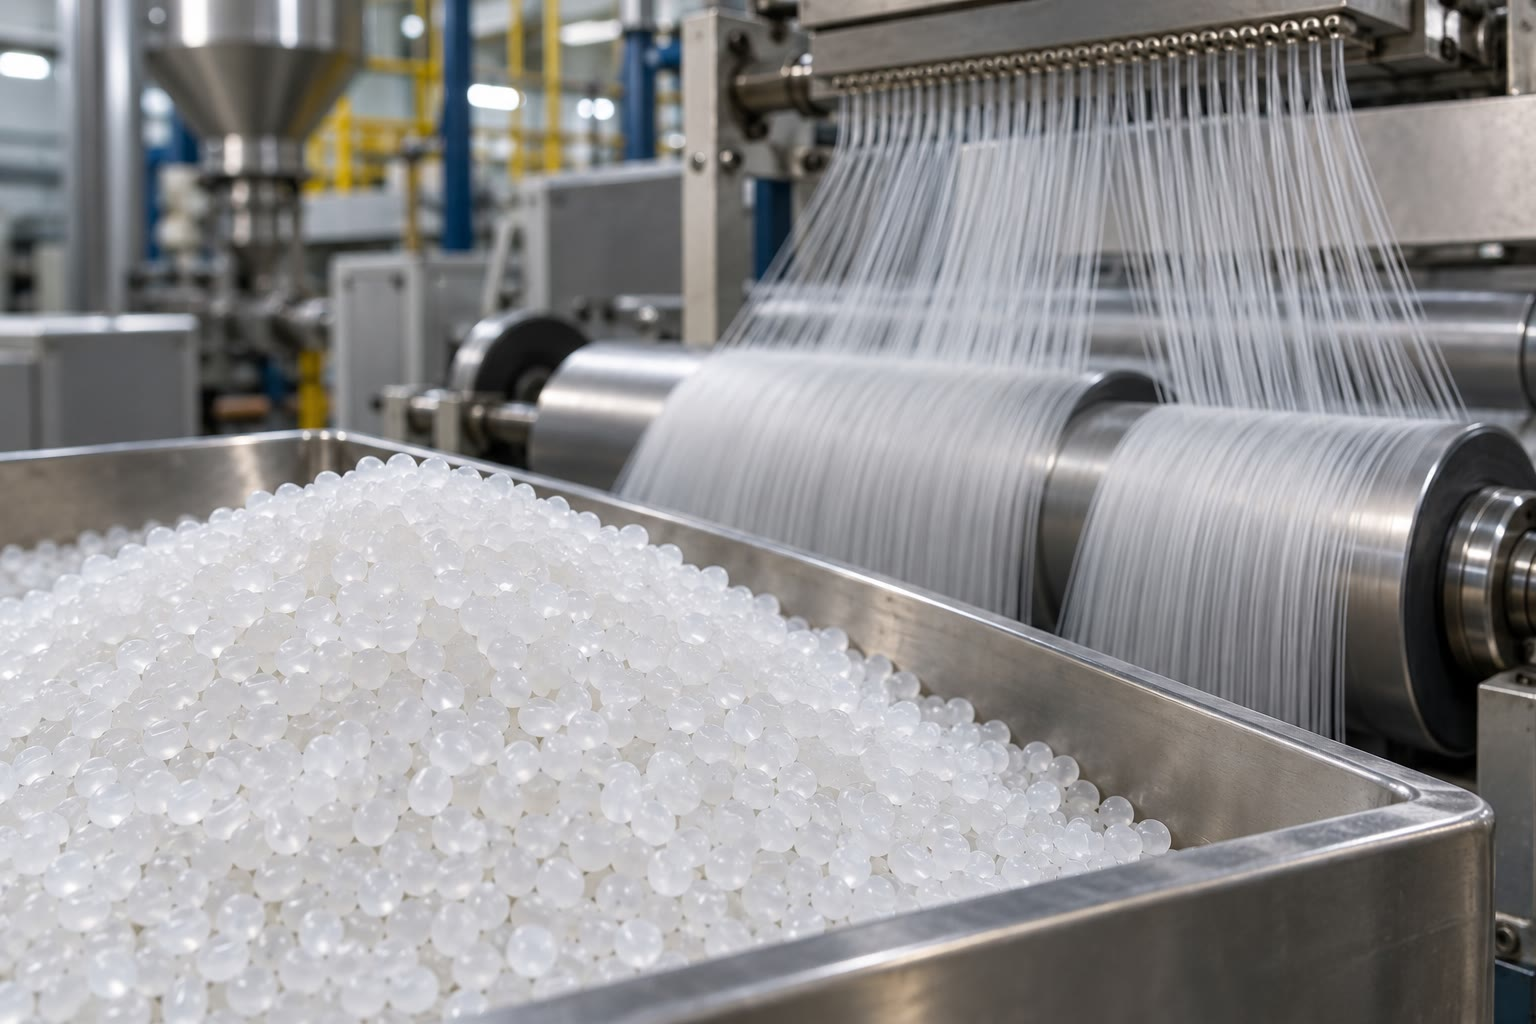
\includegraphics[width=0.58\linewidth]{images/book3/ai/b2-29-pellets.jpg}

{\small Grânulos de \omterm{def:b2:polymer-synthesis:polymer}{polímero} em uma fábrica, a forma em que os termoplásticos são vendidos, e fibras
sendo estiradas de uma fieira sobre rolos giratórios atrás deles (ilustração).}
\end{omfigure}

\begin{history}[Um rendimento de 99~\% não basta]
\begin{minipage}[t]{0.2\linewidth}
\vspace{0pt}
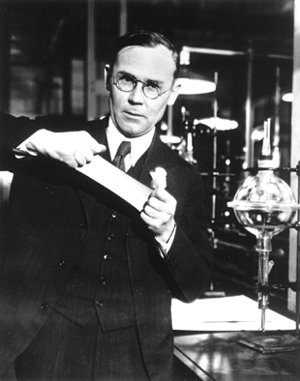
\includegraphics[width=\linewidth]{images/book3/carothers.jpg}
\end{minipage}\hfill
\begin{minipage}[t]{0.76\linewidth}
\vspace{0pt}
Wallace Carothers, jovem professor universitário recrutado por um laboratório industrial para fazer
pesquisa fundamental, construiu moléculas longas a partir de reações bem conhecidas, e seus resultados
apoiaram fortemente a ideia, então contestada, de que os \omterm{def:b2:polymer-synthesis:polymer}{polímeros} são moléculas comuns, apenas muito
longas. Sua equipe preparou poliésteres e depois, a partir de 1934, poliamidas; a equação que leva seu
nome explica por que só \omterm{def:b2:continuous-reactors:conversion}{conversões} extremas davam fibras. O náilon entrou em produção em 1939.
(Fotografia: fotógrafo desconhecido, domínio público; Wikimedia Commons.)
% ledger: hist:polyamides-1934, hist:nylon-production-1939
\end{minipage}
\end{history}

\begin{safety}{\ghs[5mm]{GHS01}\,\ghs[5mm]{GHS02}\,\ghs[5mm]{GHS05}\,\ghs[5mm]{GHS07}\,\ghs[5mm]{GHS08}\,\ghs[5mm]{GHS09}}
O estireno é inflamável e perigoso para a saúde. O peróxido de dibenzoíla é um oxidante explosivo
quando seco e é mantido úmido e fresco. A hexano-1,6-diamina e o ácido hexanodioico são corrosivos para
os olhos.
% ledger: ghs:styrene, ghs:BPO, ghs:hexanediamine, ghs:adipic-acid
\end{safety}

\section{Exercícios}

\begin{exercise}[$\star$]\label{exo:b2:polymer-synthesis:1}
Desenhe as \omterm{def:b2:polymer-synthesis:polymer}{unidades de repetição} do polieteno, do polipropeno, do poli(cloreto de vinila), do poliestireno e do náilon-6,6.
\end{exercise}

\begin{exercise}[$\star$]\label{exo:b2:polymer-synthesis:2}
Crescimento em etapas ou em cadeia: PET a partir do etano-1,2-diol e do ácido benzeno-1,4-dicarboxílico;
poliestireno; náilon-6,6; poli(metacrilato de metila); poli(ácido lático) a partir do ácido
2-hidroxipropanoico?
\end{exercise}

\begin{exercise}[$\star$]\label{exo:b2:polymer-synthesis:3}
Um poliestireno tem $\bar X_n = 1000$. Calcule $\bar M_n$, desprezando os grupos terminais.
\end{exercise}

\begin{exercise}[$\star$]\label{exo:b2:polymer-synthesis:4}
Uma cadeia de polipropeno desenhada em zigue-zague plano tem seus grupos metila do lado do leitor,
depois afastados, depois voltados para ele, depois afastados, e assim por diante. Dê sua \omterm{def:b2:polymer-synthesis:tacticity}{taticidade}.
Ela poderia cristalizar?
\end{exercise}

\begin{exercise}[$\star\star$]\label{exo:b2:polymer-synthesis:5}
Uma amostra é uma mistura de massas iguais de duas frações, de massas molares \qty{10}{kg/mol} e
\qty{100}{kg/mol}. Calcule $\bar M_n$, $\bar M_w$ e a \omterm{def:b2:polymer-synthesis:averages}{dispersidade}.
\end{exercise}

\begin{exercise}[$\star\star$]\label{exo:b2:polymer-synthesis:6}
Calcule $\bar X_n$ para uma \omterm{def:b2:polymer-synthesis:step-chain}{polimerização em etapas} equilibrada com $p = 0.98$ e $p = 0.995$.
\end{exercise}

\begin{exercise}[$\star\star$]\label{exo:b2:polymer-synthesis:7}
Um diácido e uma diamina são misturados com um excesso de 1~\% (em mols) da diamina. Qual é o maior
$\bar X_n$ que se pode atingir?
\end{exercise}

\begin{exercise}[$\star\star$]\label{exo:b2:polymer-synthesis:8}
Em uma polimerização radicalar, a concentração de iniciador é dobrada. Por que fator mudam a velocidade
de polimerização e o \omterm{def:b2:polymer-synthesis:chain-length}{comprimento de cadeia cinético}?
\end{exercise}

\begin{exercise}[$\star\star$]\label{exo:b2:polymer-synthesis:9}
O poli(cloreto de vinila) é rígido; as mangueiras de jardim feitas dele são flexíveis porque contêm um
plastificante, uma pequena molécula misturada entre as cadeias. Explique pela transição vítrea.
\end{exercise}

\begin{exercise}[$\star\star\star$]\label{exo:b2:polymer-synthesis:10}
Mostre que a distribuição mássica de Flory $w_x = x(1-p)^2p^{\,x-1}$, vista como função de um $x$
contínuo, é máxima em $x = -1/\ln p$, e que este valor é próximo de $\bar X_n$ quando $p$ é próximo de 1.
\end{exercise}

\begin{exercise}[$\star\star\star$]\label{exo:b2:polymer-synthesis:11}
O PET é preparado em duas fases: o benzeno-1,4-dicarboxilato de dimetila com excesso de etano-1,2-diol
dá o benzeno-1,4-dicarboxilato de bis(2-hidroxietila) e metanol; depois esse diéster é aquecido sob
vácuo e polimeriza, liberando etano-1,2-diol. Escreva as duas fases e explique como a segunda fase
resolve o problema estequiométrico da equação de Carothers.
\end{exercise}

\begin{exercise}[$\star\star\star$]\label{exo:b2:polymer-synthesis:12}
Em uma copolimerização radicalar dos \omterm{def:b2:polymer-synthesis:polymer}{monômeros} 1 e 2, a composição instantânea do \omterm{def:b2:polymer-synthesis:copolymer}{copolímero} é
dada por $\dfrac{\mathrm d[\mathrm M_1]}{\mathrm d[\mathrm M_2]} = \dfrac{[\mathrm M_1](r_1[\mathrm M_1]
+ [\mathrm M_2])}{[\mathrm M_2]([\mathrm M_1] + r_2[\mathrm M_2])}$, onde $r_1$ e $r_2$ são as
razões de reatividade (dados do exercício: $r_1 = 2.0$, $r_2 = 0.5$). Calcule a razão das unidades no
\omterm{def:b2:polymer-synthesis:copolymer}{copolímero} formado a partir de uma alimentação equimolar. O que acontece se $r_1 = r_2 = 0$?
\end{exercise}

\section{Problema: Náilon-6,6 aos quilos}

\begin{problem}[{Problema de fim de semana --- os monômeros e o sal de náilon, a equação de Carothers,
um desequilíbrio deliberado, a distribuição de Flory e a água liberada}]
\label{pb:b2:polymer-synthesis:1}
O náilon-6,6 é preparado a partir da hexano-1,6-diamina e do ácido hexanodioico. Os grupos terminais
são desprezados em todo o problema. Massas molares (\unit{g/mol}): C 12.011, H 1.008, N 14.007, O 15.999.
% ledger: aw:C, aw:H, aw:N, aw:O, ghs:hexanediamine, ghs:adipic-acid

\medskip
\noindent\textbf{Parte I --- \omterm{def:b2:polymer-synthesis:polymer}{Monômeros} e \omterm{def:b2:polymer-synthesis:polymer}{unidade de repetição}.}
\begin{enumerate}
  \item Escreva as fórmulas dos dois \omterm{def:b2:polymer-synthesis:polymer}{monômeros}.
  \item Escreva a equação da formação de uma ligação amida.
  \item Os \omterm{def:b2:polymer-synthesis:polymer}{monômeros} são primeiro combinados em um sal 1\,:\,1, cristalizado a partir de uma solução. Por quê?
  \item Dê a \omterm{def:b2:polymer-synthesis:polymer}{unidade de repetição} do náilon-6,6, sua fórmula e sua massa molar.
  \item Qual é a massa molar média $M_0$ de uma unidade proveniente de \omterm{def:b2:polymer-synthesis:polymer}{monômero} na cadeia?
  \item O que contam os dois números do nome ``6,6''?
\end{enumerate}

\medskip
\noindent\textbf{Parte II --- A equação de Carothers.}
\begin{enumerate}[resume]
  \item Calcule $\bar X_n$ e $\bar M_n$ com $p = 0.98$.
  \item O mesmo com $p = 0.99$.
  \item Explique a observação ``um rendimento de 99~\% não basta''.
  \item Que grau de avanço dá $\bar M_n = \qty{10}{kg/mol}$?
  \item Como o grau de avanço é levado tão alto na prática?
  \item Por que os \omterm{def:b2:polymer-synthesis:polymer}{monômeros} devem ser muito puros?
\end{enumerate}

\medskip
\noindent\textbf{Parte III --- Um desequilíbrio deliberado.}
\begin{enumerate}[resume]
  \item A diamina é usada com 1~\% de excesso molar. Calcule $r$.
  \item Calcule o maior $\bar X_n$ e o maior $\bar M_n$ que se podem então atingir.
  \item Calcule $\bar X_n$ com $p = 0.99$ com esse desequilíbrio.
  \item Que grupos terminam as cadeias no fim da reação?
  \item Às vezes se acrescenta um pouco de ácido etanoico. O que ele faz com as cadeias?
  \item Por que um fabricante limitaria de propósito o comprimento das cadeias?
\end{enumerate}

\medskip
\noindent\textbf{Parte IV --- Distribuição e balanço de massa.}
\begin{enumerate}[resume]
  \item Para uma mistura equilibrada com $p = 0.99$, dê a \omterm{def:b2:polymer-synthesis:averages}{dispersidade}.
  \item Calcule $\bar M_w$ com $p = 0.99$.
  \item Com $p = 0.99$, que fração das moléculas, e que fração da massa, ainda é \omterm{def:b2:polymer-synthesis:polymer}{monômero} que não
        reagiu?
  \item Perto de que comprimento de cadeia a distribuição mássica é máxima?
  \item Calcule a massa de água liberada por quilograma de náilon-6,6.
  \item Por que a fiação por fusão exige um $\bar M_n$ dentro de uma janela?
  \item Dê o grau de avanço que dá $\bar M_n = \qty{20}{kg/mol}$ para uma mistura equilibrada.
\end{enumerate}
\end{problem}
